\section{クラスタリング実験}

\subsection{実験環境}
実験にはPython3.5を用い,
機械学習のライブラリとしてTensorFlowを用いてアルゴリズムを実装した.

\subsection{精度の評価}
クラスタリング精度の評価はPythonのライブラリであるscilit-learnを用い,以下の3項目により行う.
\begin{description}
  \item[ARI; Adjusted Rand Index, 調整ランド指数]
    クラスタの正解ラベルに対してクラスタリング結果の一致度を評価する指標.1に近づくほどよい結果.
  \item[NMI; Normalized Mutual Information, 正規化相互情報量]
    相互情報量を正規化した尺度.
  \item[Purity]
    生成されたクラスタがどれだけ多数派で占められているかを表す尺度
\end{description}

\subsection{X-meansによるクラスタリング}
K-meansと同様に,クラスタ数が5つのデータを生成し,X-meansにより分割した結果,
\figref{img:xmeans-after}のようになった.
図より,クラスタ数を5つとして適切にクラスタリングを行っていることがわかる.

\begin{figure}[htbp]
  \begin{center}
    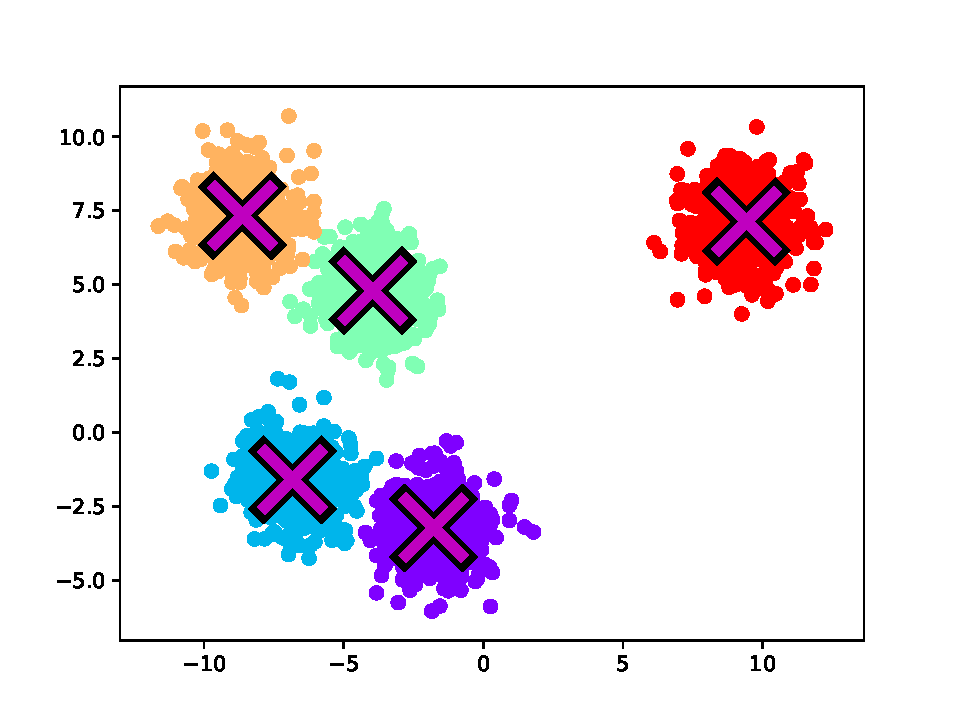
\includegraphics[width=0.8\linewidth]{img/x-means/after.pdf}
    \caption{X-meansによるクラスタリング結果}
    \label{img:xmeans-after}
  \end{center}
\end{figure}
